\documentclass{article}


\usepackage{arxiv}

\usepackage[utf8]{inputenc} % allow utf-8 input
\usepackage[T1]{fontenc}    % use 8-bit T1 fonts
\usepackage{hyperref}       % hyperlinks
\usepackage{url}            % simple URL typesetting
\usepackage{booktabs}       % professional-quality tables
\usepackage{amsfonts}       % blackboard math symbols
\usepackage{nicefrac}       % compact symbols for 1/2, etc.
\usepackage{microtype}      % microtypography
\usepackage{lipsum}
\usepackage{amsmath}
\usepackage{amsthm}
\usepackage{graphicx}

\title{Project in BMML: Team with bayesian flavor}


\author{
   \And
  Dmitriy Salnikov   \\
  Skolkovo Institute of Science and Technology \\
  Moscow, Russia \\
   \And
  Aliaksandr Nekrashevich \\
  Skolkovo Institute of Science and Technology \\
  Moscow, Russia \\
   \And
  Nurlan Shagadatov\\
  Skolkovo Institute of Science and Technology \\
  Moscow, Russia \\
}

\newtheorem{definition}{Definition}
\newtheorem{theorem}{Theorem}
\begin{document}
\maketitle

% keywords can be removed
\keywords{GAN, deep learning, optimal transport, VAE, variational autoencoder, autoencoder, generative adversarial network}


\section{Introduction}

Throughout recent years, there's been a lot of research devoted to Generative models, which find a lot of applications in today's applied statistics. But in order to correctly use them you need to know what you're doing.
When evaluating their models, researchers often use latent space arithmetics to explore the latent vector space. For objects that are natural for humans(text, images) it's often argued that vectors in that space carry the semantic meaning. Thus, using such transforms in latent space leads to a natural transformation in the original space.

We study the paper \cite{main} 
exploring latent space modifications 
for generative models. The most known generative models 
are Generative Adversarial Networks (GANs) and Variational 
Auto Encoders (VAEs). The problem is that latent space operations
can create distributional mismatch, and the paper we study 
tries to resolve these mismatches with methods of 
optimal transport.

The rest of the report is organized as follows. In the 
Theoretical Explanation chapter we summarize the points presented
in the paper. In the Workflow description, we describe what 
cases and extensions we study. In the Experimental Results
chapter we present outcomes of our experiments.
Later, in Team contribution, we explain what is done by each team member. Finally, references are given.


\section{Theoretical Explanation}
As briefly mentioned in the introduction part, we are looking to correct the distributional mismatch caused by the transformation applied to the sample. To do that we construct optimal transport map, which is the solution to the Monge transporation problem. The usual way to solve it is to consider the relaxation also known as Monge-Kantorovich problem, but for the case of our interest they coincide. For more information on the OT theory refer to \cite{villani2008optimal}, \cite{peyre2017computational} for a comprehensive description. 

\begin{definition}[Monge-Kantorovich relaxation]
For a given  $c:\mathcal{X} \times \mathcal{Y} \rightarrow R^+$
$$
\inf_{p_x, p_y} \{E_{(x, y)}\sim p_{x, y} c(x, y) | (x, y) \sim p_{x, y}, x \sim p_x , y\sim p_y\}
$$
\end{definition}
Now, we will state theorems that to formulas we use. For proofs refer to \cite{main}
\begin{theorem}[Decomposition]
If probability measures $p_x, p_y$ have i.i.d components and cost function admits
$$
c(x, y) = \sum_{i=1}^{d}C(x^{i}, y^{i})
$$
Then, the solution of Monge-Kantorovich problem is component-wise i.e
$$
p^{opt}_{x, y}(x, y) = \prod_{i=1}^{d} p^{i_{opt}}_{X, Y}
$$
\end{theorem}

\begin{theorem}
If c(x, y) = h(x - y), where $h: \mathbb{R} \rightarrow \mathbb{R^+}$, then the optimal transport map from $p_x$ to $p_y$ is given by the 
$$
T_{X \rightarrow Y}(x) = F^{-1}_Y(F_X(x))
$$
Where 
\begin{itemize}
    \item $F_X$ - CDF of X
    \item $F^{-1}_Y = \inf \{ t \in \mathbb{R} | F_Y{y}(t) \ge y \}$ - pseudo-inverse CDF of Y
\end{itemize}
\end{theorem}

Then, the distributional mismatch is usually addressed in the following
steps. First, intuitive operator $y$ is constructed. Then resulting distribution is computed. 
The following table contains operations y and corresponding matched $\overline{y}$ for $\mathcal{N}(0, 1)$
\begin{table}[!h]
    \centering
    \begin{tabular}{|c|c|c|}
    \hline
        2-point interpolation & $y = tz_1 + (1 - t)z_2$ & $\overline{y} = \frac{y}{\sqrt{(1 - t)^2 + t^2}}$  \\
        \hline
        n-point interpolation & $y = \sum_{i=1}^{n}t_i z_i, \sum_{i=1}t_i=1$ 
         & $\overline{y} = \frac{y}{\sqrt{\sum_{i=1}^{n}t_i^2}}$ \\
         \hline
         vicinity sampling & $y = y_0 + \varepsilon u, u \sim N(0, I)$ & $\overline{y} = \frac{y}{\sqrt{1 + \varepsilon^2}}$ \\
         \hline
         analogies & $y = z_3 + (z_2 - z_1)$ & $\overline{y} = \frac{y}{\sqrt{3}}$ \\
         \hline
    \end{tabular}
    \caption{Operations and distribution preserving maps for $\mathcal{N}(0, 1)$}
    \label{tab:my_label_1}
\end{table}

\section{Workflow Desription}
We have separated the project into three parts:

\begin{enumerate}
    \item Reproducing the paper. This part is dedicated to GANs. 
        Here we train and adopt DCGAN,
        compute inception score, evaluate results on 
        different datasets.

    \item Applying distribution matching for VAE. Here, we work
        only with interpolation models.

    \item Correcting missing values for VAE. We take 
        initial image, corrupt it in different way, 
        and then reconstruct 
        it using optimal transport distribution matching.
\end{enumerate}

\section{Experimental Setup}
\subsection{Data description}
To evaluate and compare our models we use 3 freely available datasets used to train and assess generative models:
\begin{itemize}
    \item LSUN-bedrooms - collection of images of bedrooms
    \item CelebA - collection of celebrity face photos
    \item LLD - collection of logo pictures
\end{itemize}

\subsection{Quality assessment}
We compare initial and matched distributions using two approaches
\begin{itemize}
    \item Qualitative results: Since we obtain images by using the generator, we can just look at them and tell if they're looking good or natural to a human eye or not.
    \item Quantitative results: But as people doing the project, we may be biased. So as the metric that doesn't depend on our perception of the world, we use Inception Score. 
\end{itemize}
For a given generator the inception score is just
    $$
    \exp{E_{p_x}KL(p(y|x) || p(y))}, p_x \sim G \text{ where } p(y) = \int p(y|x)p_g(x) dx \approx \frac{1}{N}\sum_{i=1}^{N} p(y_i|x_i) \text{; where } x_i \sim G
    $$
    
\subsection{DCGAN and VAE models}
We use images of size 64x64 and latent space size 100 for the training of DCGAN model, 45x45 deep-funneled images and latent space of size 100 for training of VAE. There is a need to note that for the uniform prior we could not obtain the good model for GAN, so we focus more on Normal distribution.

\section{Results}
\subsection{2 point interpolation}

\begin{center}
\begin{figure}
    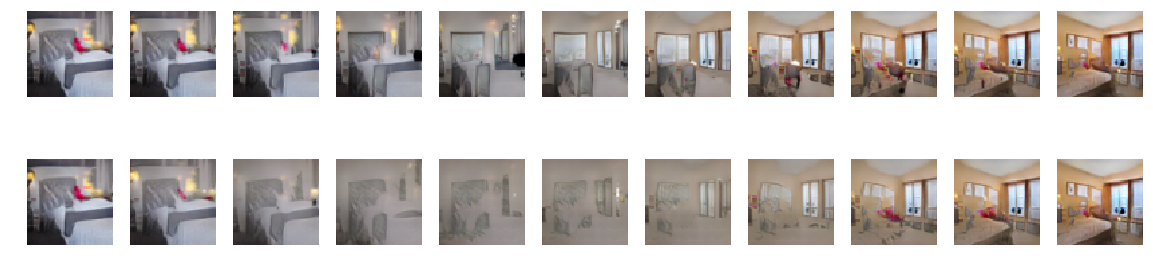
\includegraphics[width=\linewidth]{CelebA/images/LSUN_int2_2.png}
    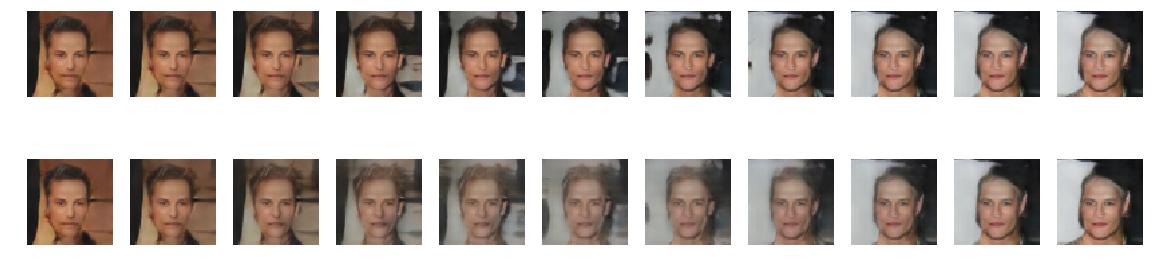
\includegraphics[width=\linewidth]{CelebA/images/CelebA_int2_5.png}
    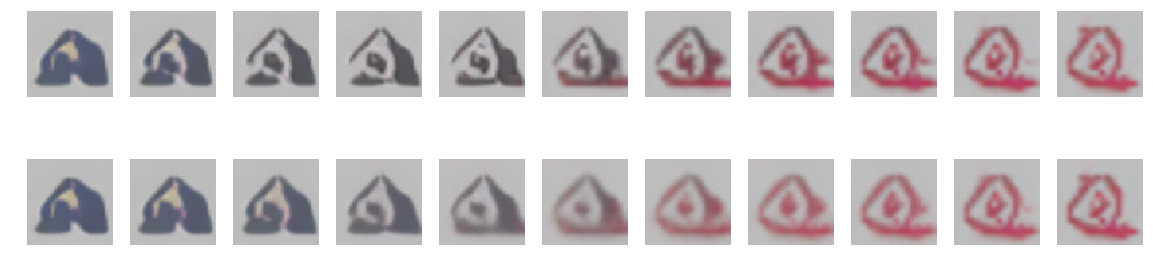
\includegraphics[width=\linewidth]{CelebA/images/LLD_int2_3.png}
    \caption{2 point interpolation}
\end{figure}
\end{center}
We begin with the classic example of 2-point interpolation: Figure 1 shows
three examples per dataset for an interpolation between 2 points in latent space. Each example is first done via matched interpolation (upper raw), then with linear interpolation(lower raw). It is immediately obvious that linear interpolation produces inferior results with generally more blurry, less saturated and less detailed output images. Differences between the two types of interpolation methods for CelebA are much more subtle to the point that they are virtually indistinguishable when viewed side-by-side. This is not an inconsistency though: while distribution mismatch can cause large differences, it can also happen that the model generalizes well enough that it does not matter.
\subsection{4 point interpolation}
An even stronger effect can be observed when we do 4-point interpolation,
showcased in Figure 2 (LSUN) and Figure 4 (LLD icons). The higher resolution of the LSUN output highlights the very apparent loss of detail and increasing prevalence of artifacts towards the midpoint in the linear version, compared to matched interpolation.



\begin{center}
\begin{figure}
    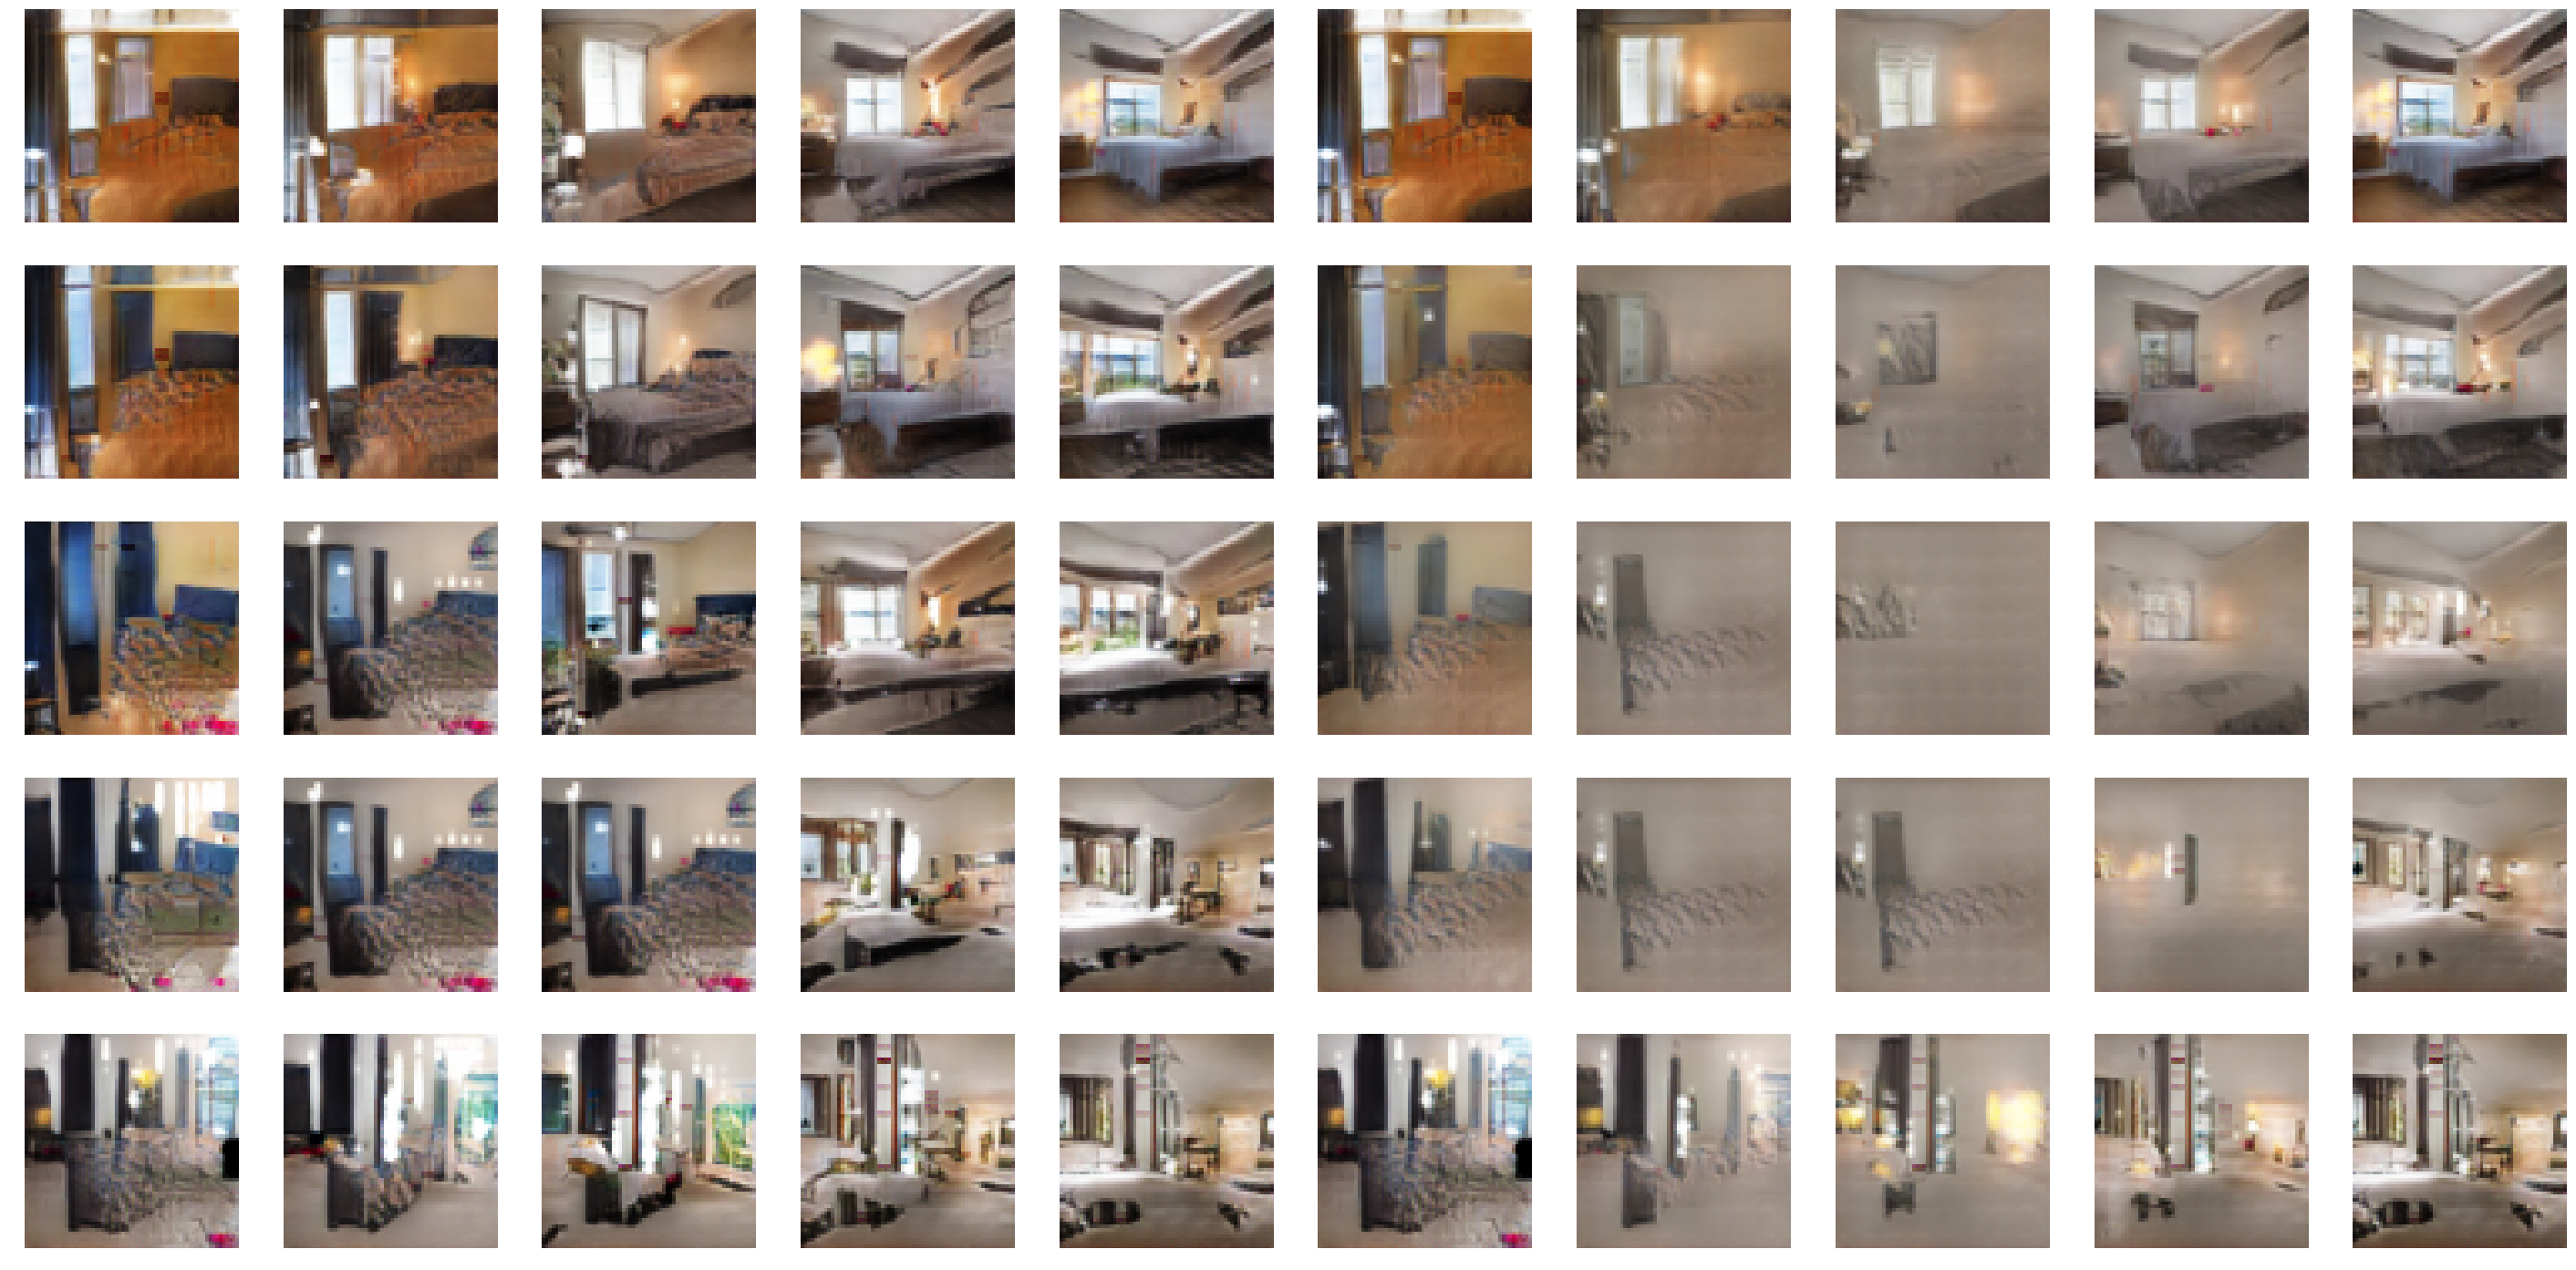
\includegraphics[width=\linewidth]{CelebA/images/LSUN_int4_1.png}
    \caption{4 point interpolation (LSUN)}
\end{figure}
\end{center}

\begin{center}
\begin{figure}
    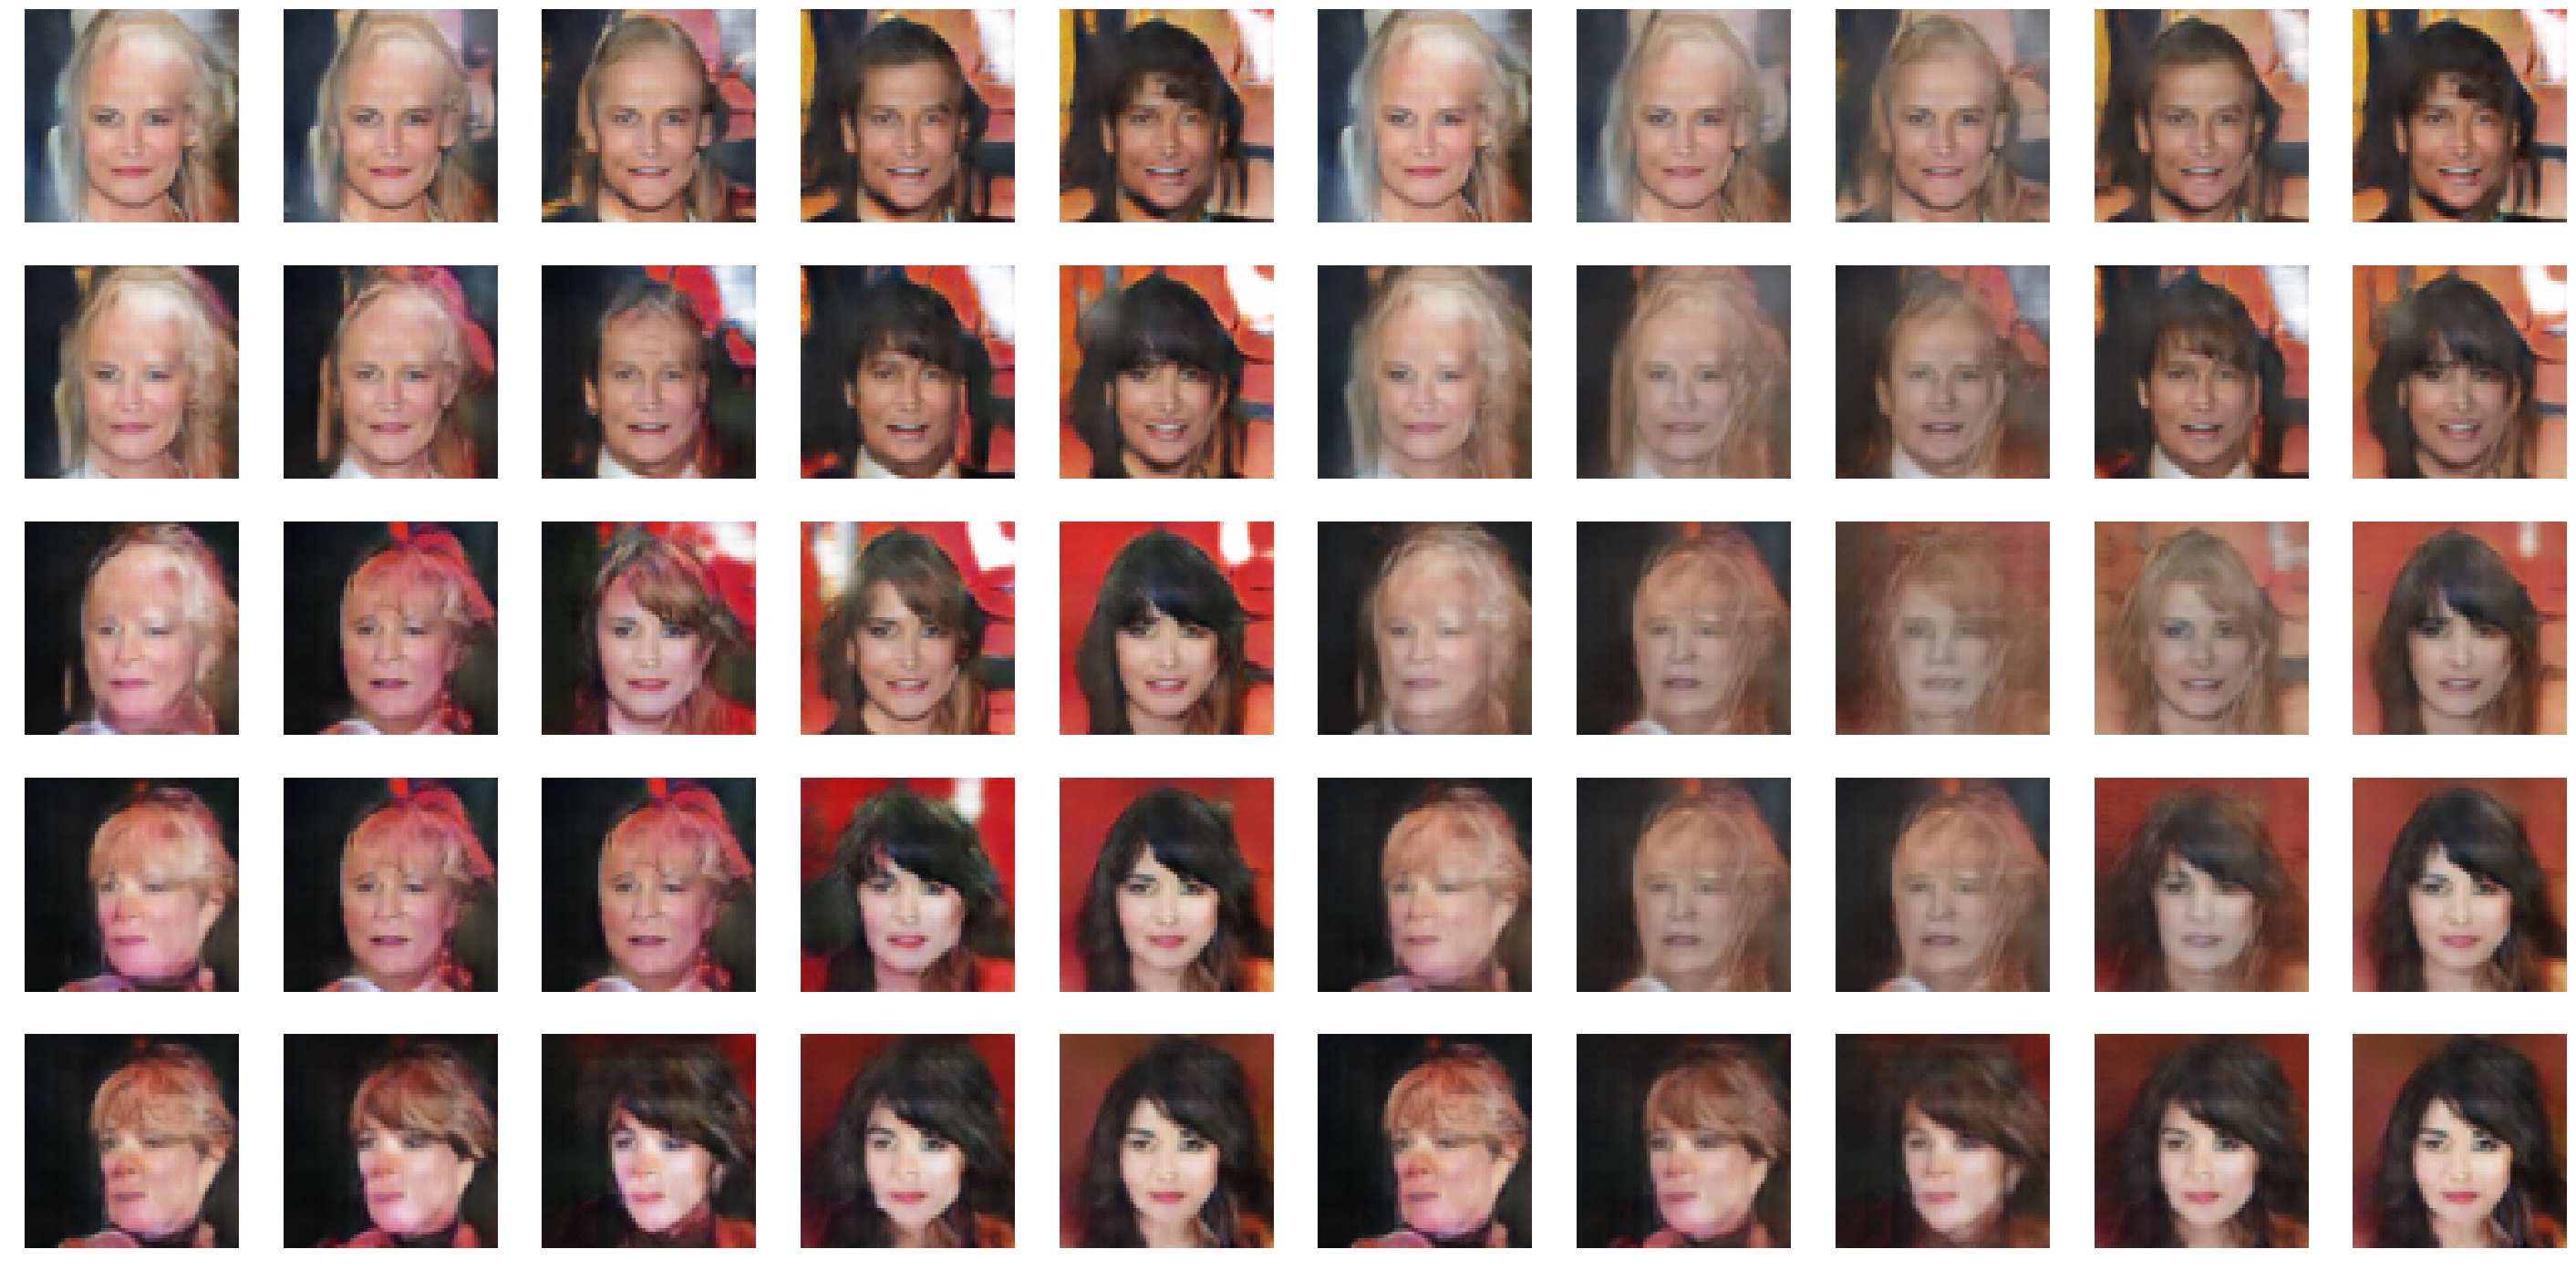
\includegraphics[width=\linewidth]{CelebA/images/CelebA_int4_2.png}
    \caption{4 point interpolation (CelebA)}
\end{figure}
\end{center}

\begin{center}
\begin{figure}
    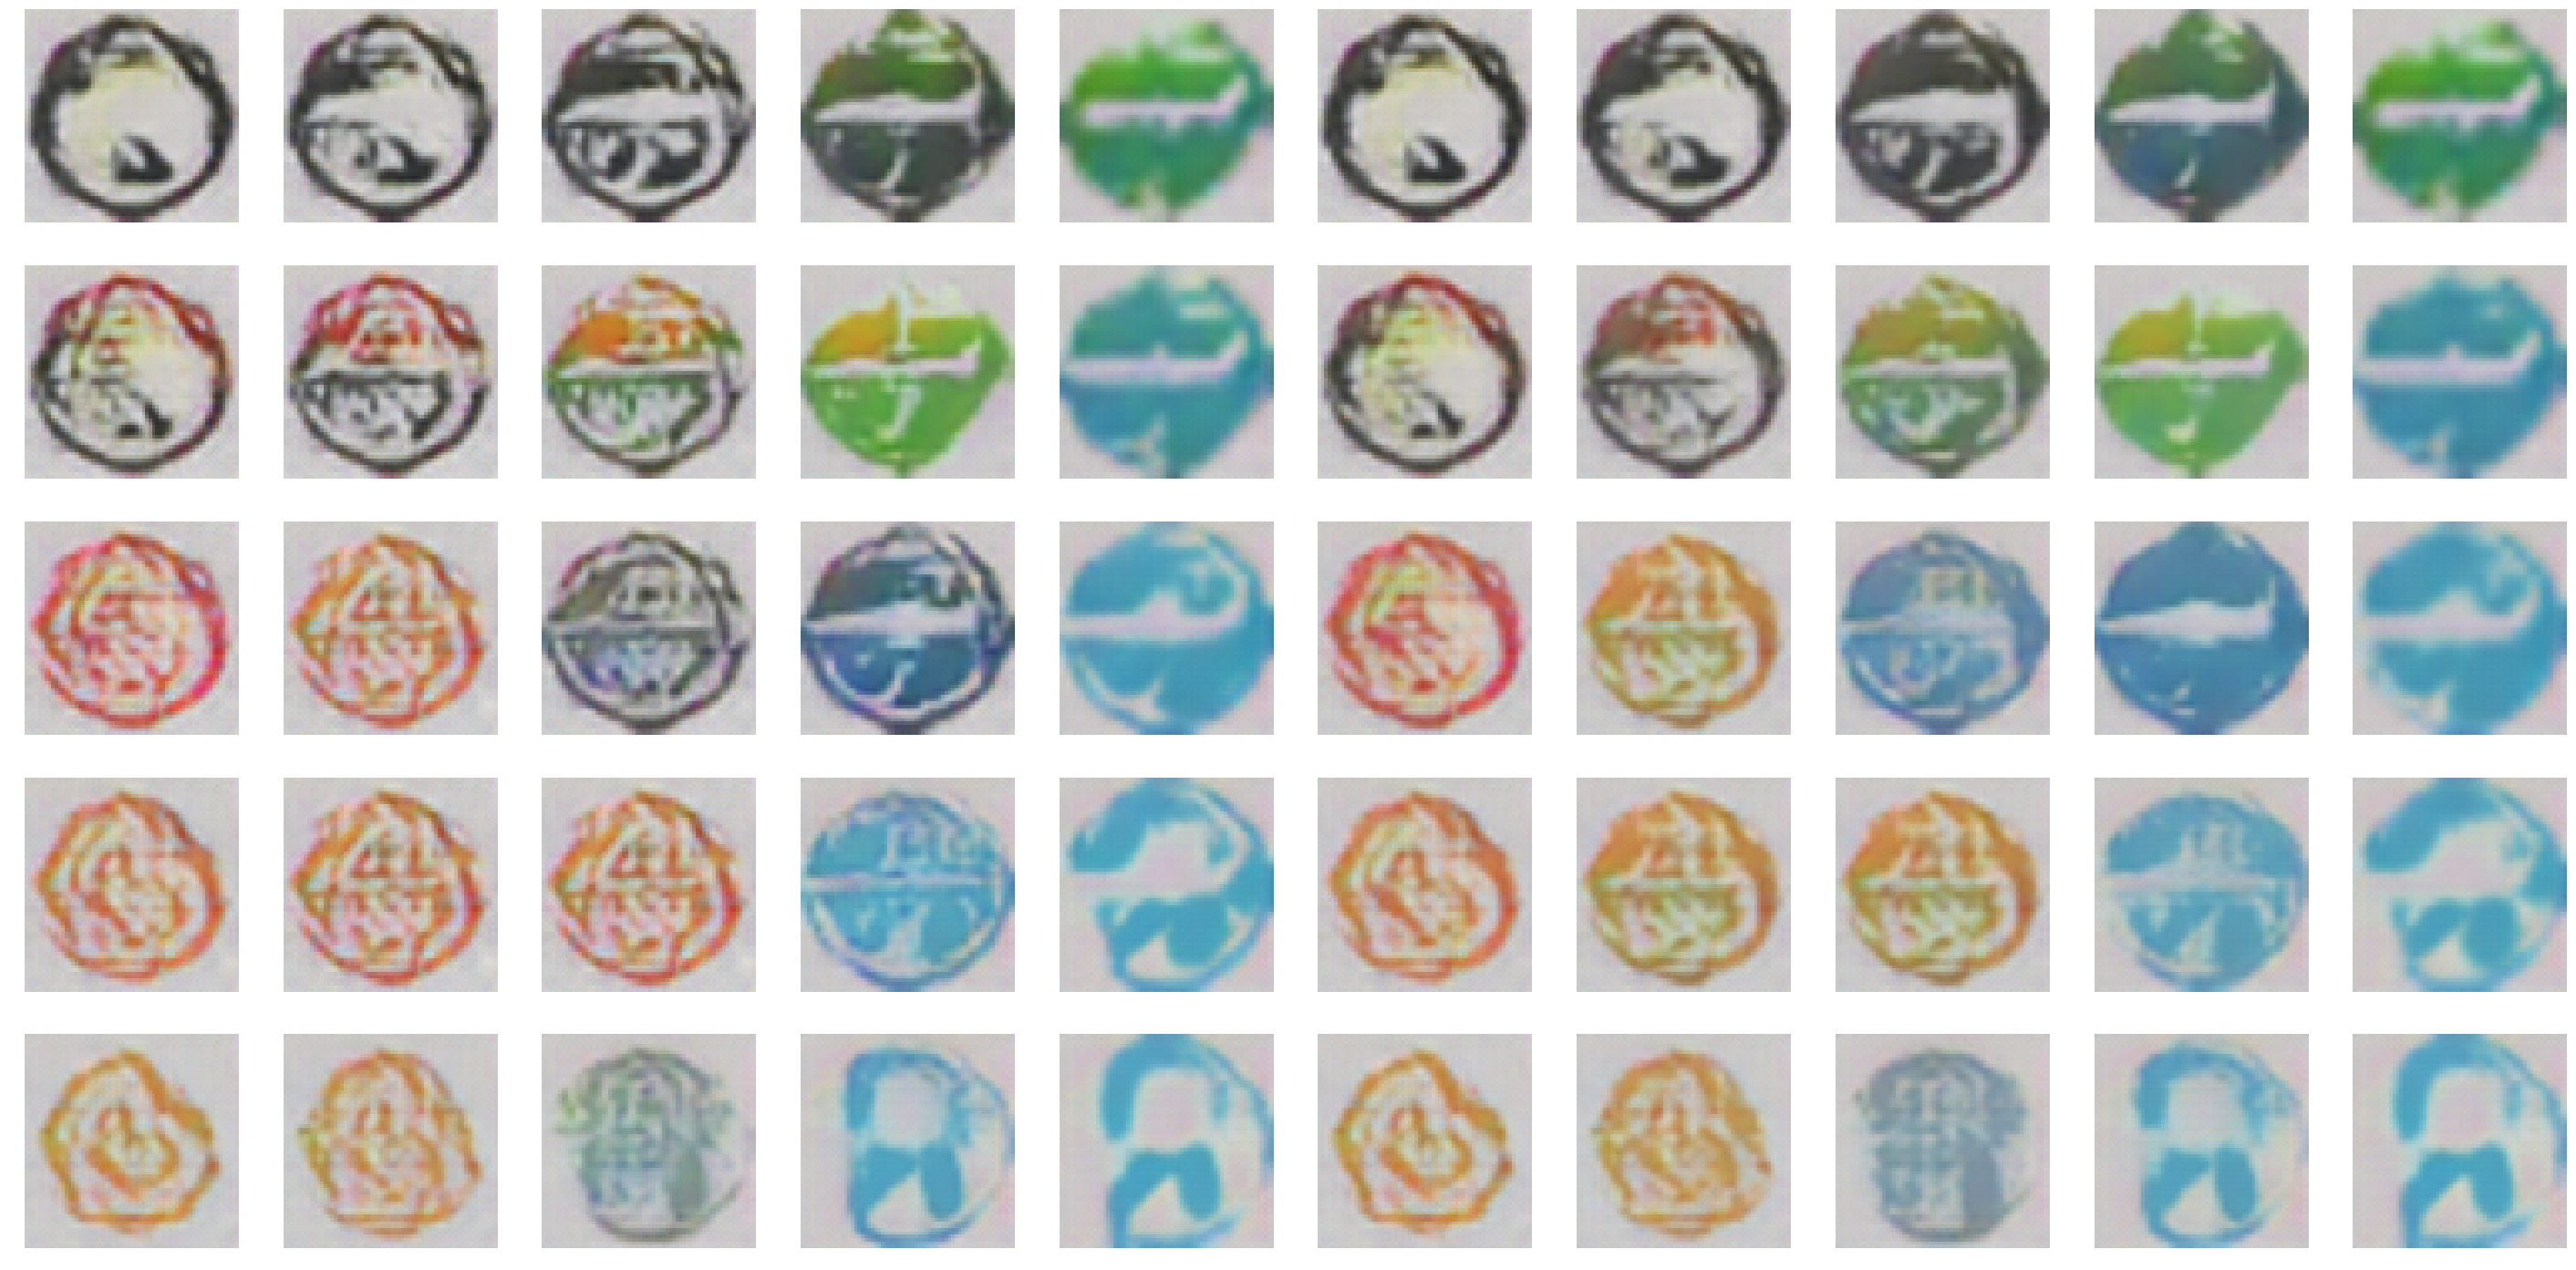
\includegraphics[width=\linewidth]{CelebA/images/LLD_int4_1.png}
    \caption{4 point interpolation (LLD icon)}
\end{figure}
\end{center}


\subsection{Random walk (vicinity sampling)}
An interesting property of matched vicinity sampling is that we can obtain a
random walk in the latent space by applying it repeatedly: we start at a point $y_0 = z$ drawn from the prior, and then obtain point $y_i$ by sampling a single point in the vicinity of $y_{i-1}$ , using some fixed ’step size’ $\varepsilon$ .We show an example of such a walk in Figure 5, using $\varepsilon$ = 0.5. As a result of the repeated application of the vicinity sampling operation, the divergence from the prior distribution in the non-matched
case becomes stronger with each step, resulting in completely unrecognizable output images on the LSUN and LLD icon models. Even for the CelebA model where differences where minimal be-
fore, they are quite apparent in this experiment. The random walk thus perfectly illustrates the need for respecting the prior distribution when performing any operation in latent space, as the adverse effects can cumulate through the repeated application of operators that do not comply to the prior distribution.

\begin{center}
\begin{figure}
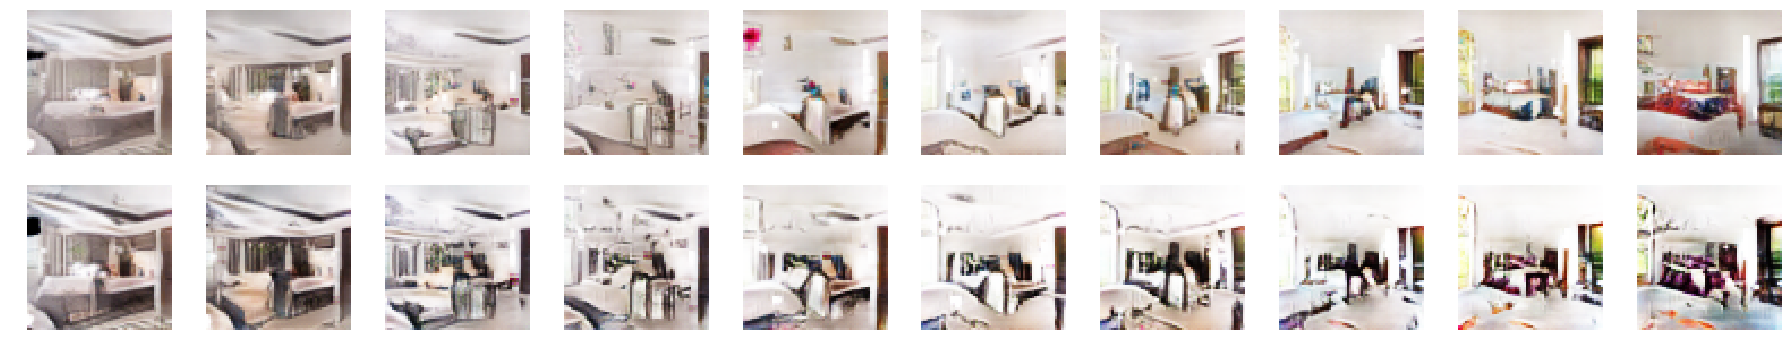
\includegraphics[width=\linewidth]{CelebA/images/LSUN_rw_2.png}\\
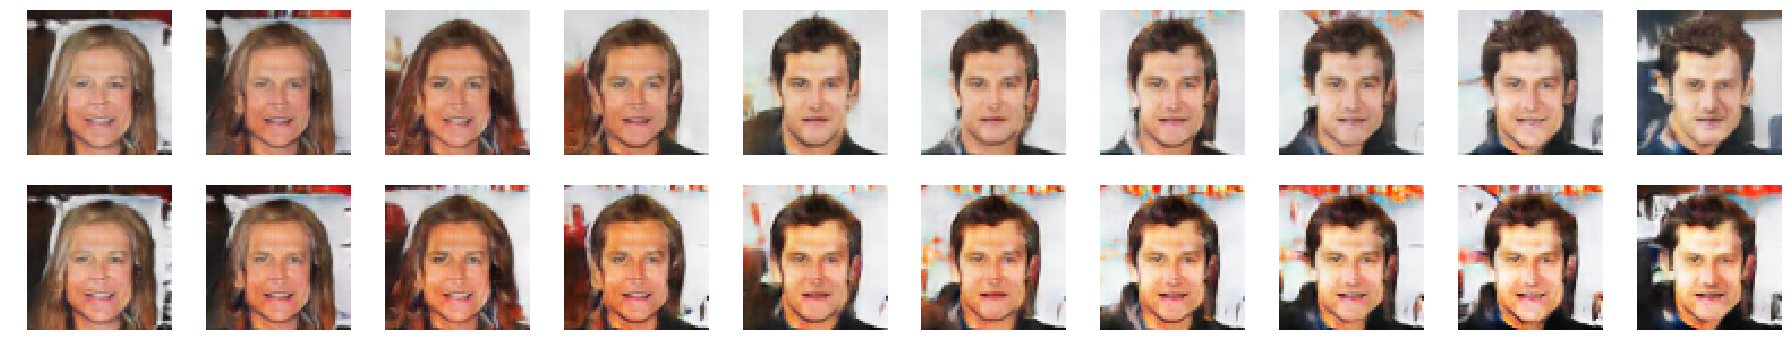
\includegraphics[width=\linewidth]{CelebA/images/Celeba_rw_2.png}\\
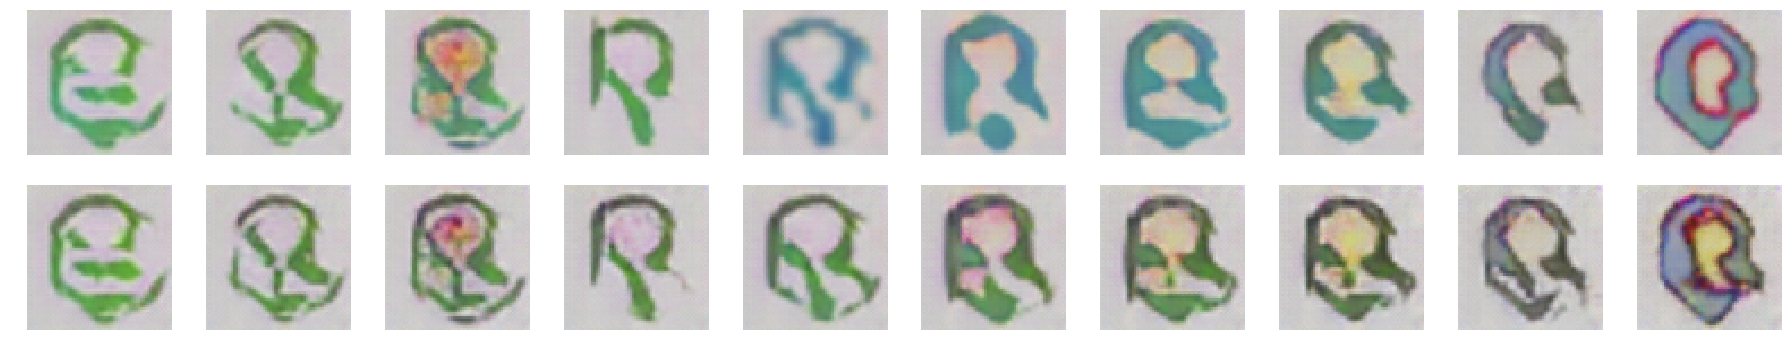
\includegraphics[width=\linewidth]{CelebA/images/LLD_rw_1.png}
\caption{Random walks through latent space}
\end{figure}
\end{center}

\subsection{Inception score}
In order to quantitatively confirm the observations of the previous subsection, we computed the Inception score of our trained models (i.e. using random samples from the prior). More precisely, we sampled midpoints from 2-point interpolation and 4-point interpolation described above with 5000 samples and computed the mean value of Inception Score.  Compared to the original scores of the trained models, matched operations are statistically indistinguishable (as expected) while the linear interpolation gives a significantly lower score in all settings.
\begin{table}[]
    \centering
    \begin{tabular}{|c |c |c |c |}
    \hline
    & CelebA & LSUN & LLD \\
    \hline
        Usual 2-point & 1.799 & 1.448 & 1.699\\
    \hline
        Matched 2-point & 2.008 & 1.662 & 2.130\\
    \hline
        Usual 4-point & 1.206 & 1.370 & 1.658\\
    \hline
        Matched 4-point & 2.052 & 2.128 & 3.285\\
    \hline
    \end{tabular}
    \caption{2 point interpolation inception score}
    \label{tab:my_label_2}
\end{table}
\subsection{VAE results}
In addition, we conducted the same experiments for Variational Autoencoder trained on Labelled Faces in the Wild Dataset. Unfortunately, the difference between linear and matched interpolations is not obvious, although in some cases the exact interpolation generates clearer (under trained decoder conditions) images. Eventually, we attempted to reconstruct corrupted image using interpolations. Precisely, we took initial image from dataset and corrupted by changing canals of some pixels and reconstructed midpoint interpolation between two latent vectors corresponding to corrupted images. In this case also results are not satisfactory. 



\begin{center}
\begin{figure}
    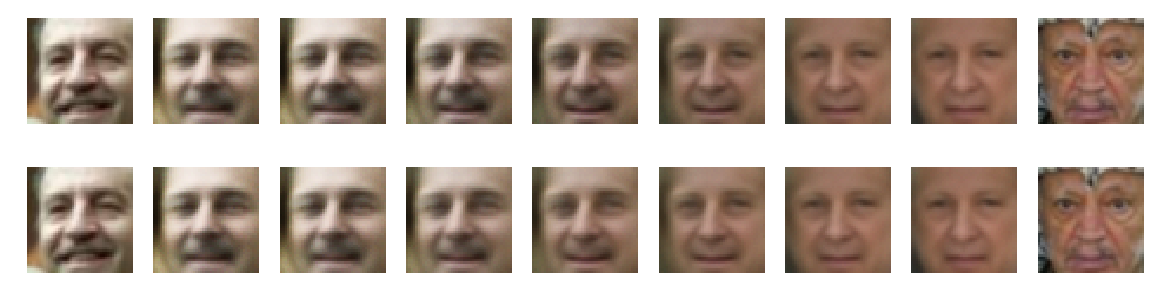
\includegraphics[width=\linewidth]{report/vae_int2_1.png}
    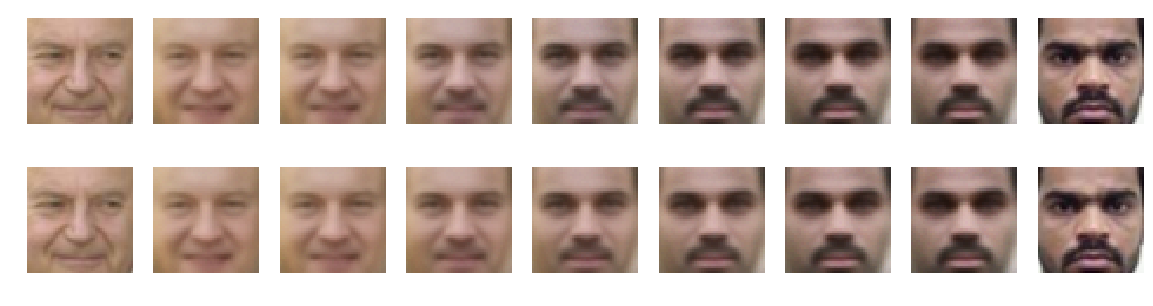
\includegraphics[width=\linewidth]{report/vae_int2_2.png}
    \caption{VAE 2-point interpolation}
\end{figure}
\end{center}

\begin{center}
\begin{figure}
    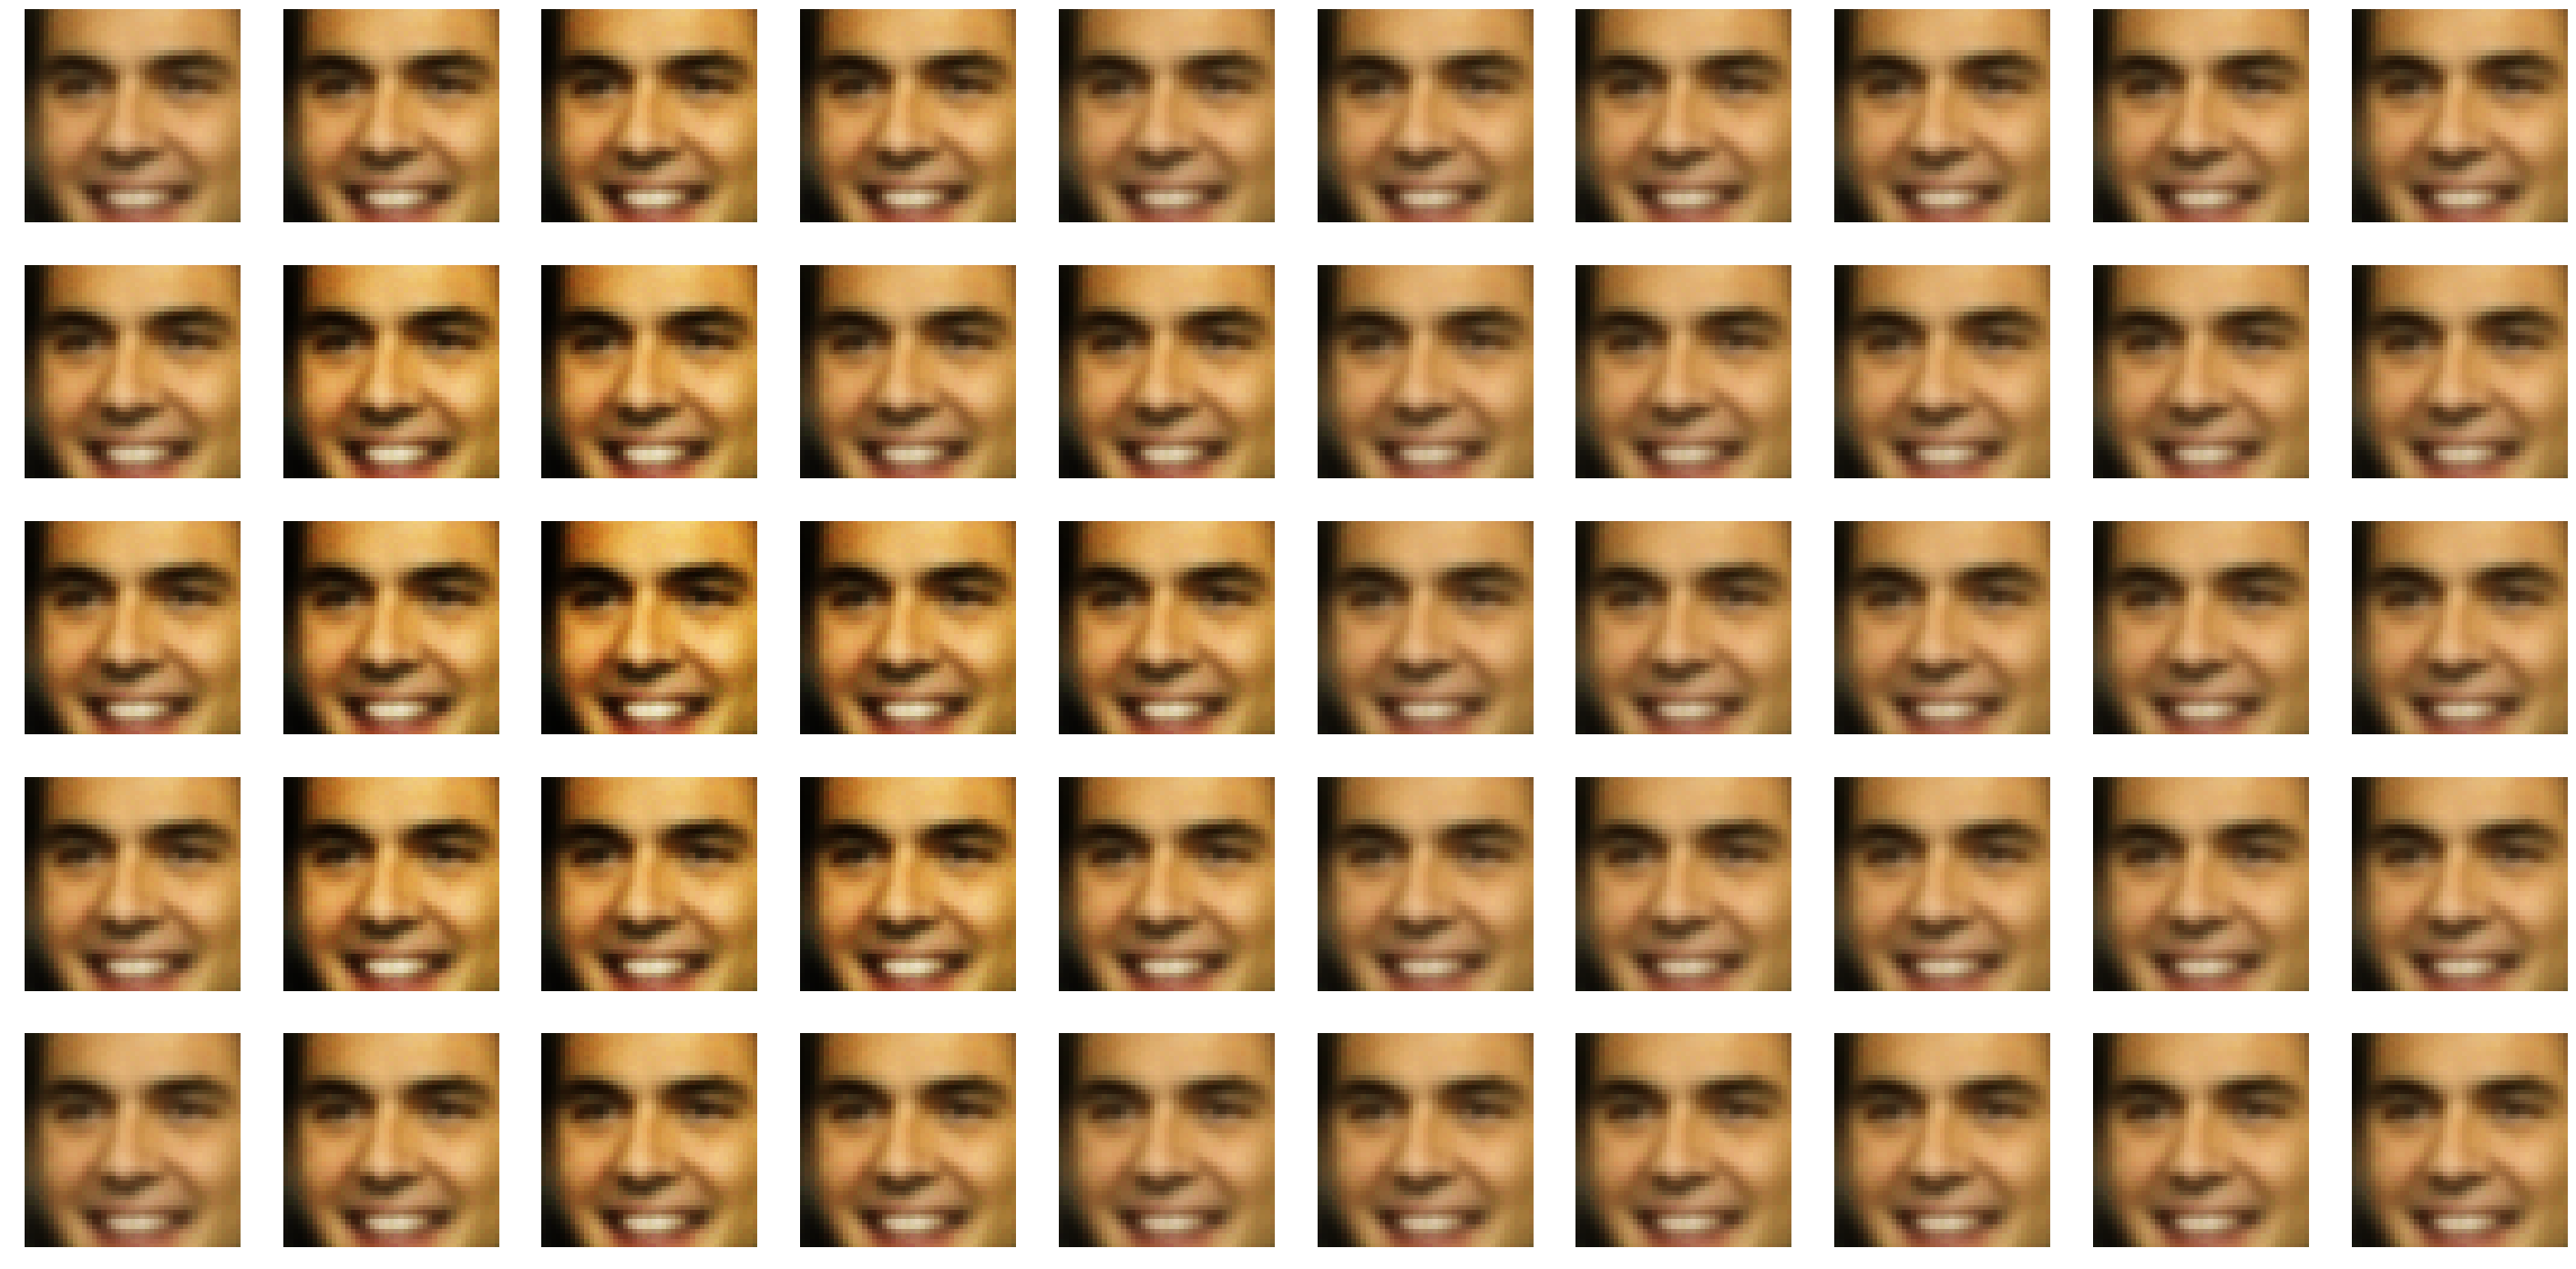
\includegraphics[width=\linewidth]{report/vae_int4.png}
    \caption{VAE 4-point interpolation}
\end{figure}
\end{center}

\begin{center}
\begin{figure}
    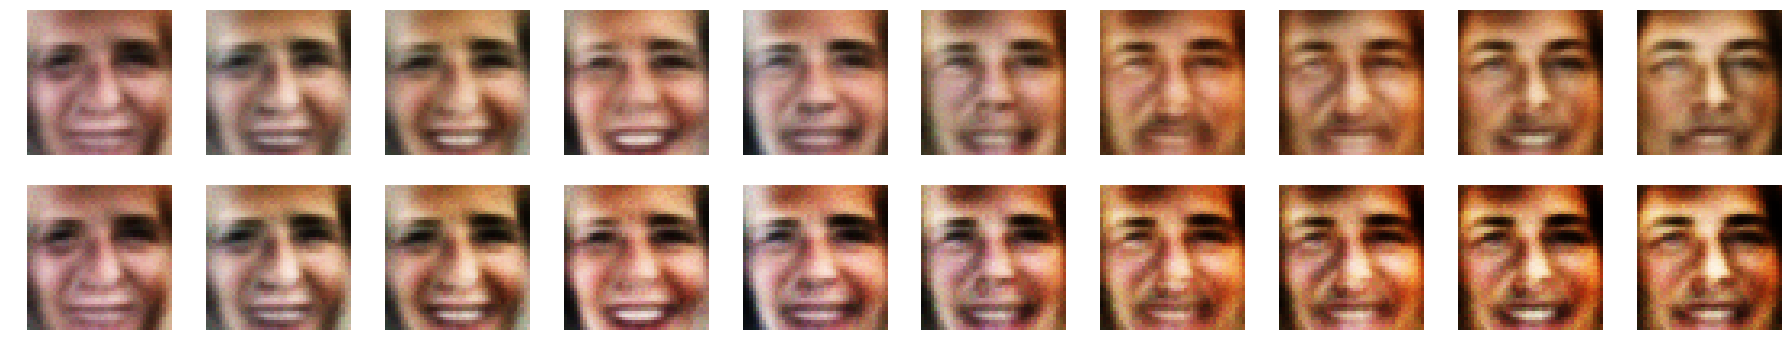
\includegraphics[width=\linewidth]{report/vae_rw.png}
    \caption{VAE random walk (vicinity sampling)}
\end{figure}
\end{center}

\begin{figure}%
\centering
\subfigure{%
\label{fig:first}%
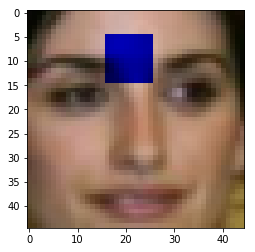
\includegraphics[height=1in]{report/vae_mi.png}}
\qquad
\subfigure{%
\label{fig:second}%
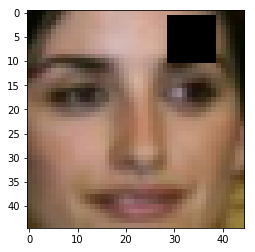
\includegraphics[height=1in]{report/vae_missing_1.png}}
\caption{Corrupted images}
\end{figure}

\begin{center}
\begin{figure}
    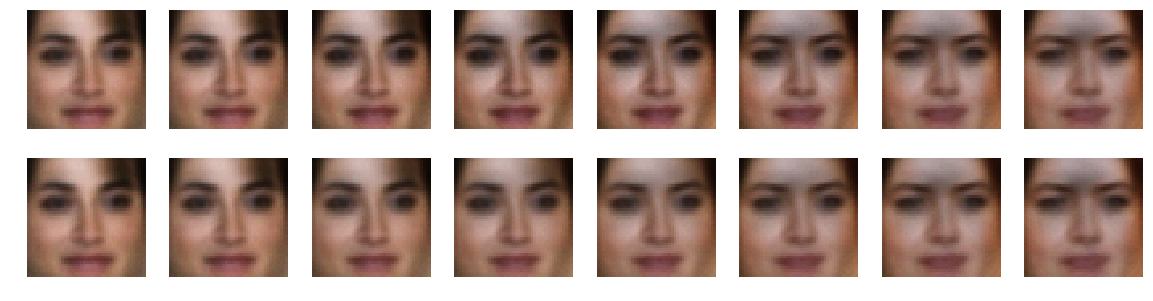
\includegraphics[width=\linewidth]{report/vae_missing_3.png}
    \caption{VAE missing value reconstruction}
\end{figure}
\end{center}

\section{Conclusions}
We notice that it the impact that distribution mismatch has on the result depends on how well the generator is fitted. For the biggest dataset LSUN, we obtain a very good generator, which is very sensitive to the mismatch. If the generator is not that good, the mismatch does not introduce that big of a change, as we can see on examples of VAE or DCGAN on LLD dataset.


\section{Team contribution}
\begin{enumerate}
        \item Dmitriy Salnikov: DCGAN experiments,
            distribution matching operations, presentation,
            team management, theoretical part of the paper
        \item Aliaksandr Nekrashevich: VAE experiments,
            inception score for DCGANs, report
        \item Nurlan Shagadatov: DCGAN experiments, VAE experiments, presentation
\end{enumerate}

\bibliographystyle{unsrt}
\bibliography{references}

\end{document}
